\documentclass[a4paper]{article}
\usepackage{graphicx}
\usepackage{bmpsize}
\usepackage{geometry}
\geometry{
	a4paper,
	includehead,
	total={170mm,257mm},
	left=20mm,
	top=20mm,
	bottom=25mm
}
\usepackage{mathpazo}
\usepackage{caption}
\captionsetup{labelfont=bf,format=hang,labelsep=period}
\usepackage{subcaption}
\usepackage{amsmath}
\usepackage{amsthm}
\usepackage[T1]{fontenc}
\usepackage{mathtools}
\usepackage{multirow,array}
\usepackage{setspace}
\onehalfspacing


\usepackage[page,toc,titletoc,title]{appendix}

\usepackage{subcaption, tzplot, asymptote, pgfplots}
\pgfplotsset{compat=1.18}
\usetikzlibrary{calc, calligraphy, decorations.pathreplacing, patterns, shapes.misc}
\usetikzlibrary{positioning}
\newcommand*\circled[1]{\tikz[baseline=(char.base)]{
		\node[shape=circle,draw,inner sep=0.2pt] (char) {#1};}}
	
\usepackage{booktabs,caption}
\usepackage[flushleft]{threeparttable}

\usepackage{xcolor}
\definecolor{main}{RGB}{0,166,82}
\definecolor{second}{RGB}{32,178,170}


\usepackage{makeidx}
\usepackage[style=apa, backend=biber, sorting=ynt, natbib=true]{biblatex}
\addbibresource{Reference(DSproject).bib}

\usepackage{mathtools}
\usepackage{sectsty}
\usepackage{titlesec}
%\titleformat{\subsubsection}
%{\normalsize\fontsize{16}{17}\itshape}{\thesubsubsection}{1em}{}
\usepackage{amssymb}
%\usepackage[dvipsnames]{xcolor}
\usepackage[skins]{tcolorbox}

%\usepackage{tikz}

%\usepackage{tzplot}
%\usetikzlibrary{positioning}

\usepackage{varwidth}
\usepackage{pifont} %itemize bullet style
\usepackage{enumitem}
\usepackage[english]{babel}
\usepackage[utf8]{inputenc}

\usepackage{float}
\usepackage{hyperref}
\hypersetup{
	colorlinks=true,
	linkcolor=blue,
	filecolor=blue,      
	urlcolor=blue,
	citecolor=blue
}


\theoremstyle{definition}
\newtheorem{theorem}{Theorem}[section]
\newtheorem{example}{Example}[section]
\newtheorem{prop}{Proposition}[section]
\newtheorem{corollary}{Corollary}[section]
\newtheorem{lemma}[theorem]{Lemma}
\theoremstyle{definition}
\newtheorem{definition}{Definition}[section]
\theoremstyle{remark}
\newtheorem*{remark}{Remark}
\newenvironment{solution}{\renewcommand{\proofname}{Solution}\begin{proof}}{\end{proof}}
\renewcommand\qedsymbol{$\blacksquare$}

\sectionfont{\fontsize{16}{15}\selectfont}
\subsectionfont{\fontsize{14}{15}\selectfont}
\subsubsectionfont{\fontsize{13}{15}\selectfont}
\setlength{\jot}{12pt}
\DeclareMathOperator*{\plim}{plim}
%\numberwithin{equation}{section}
%\renewcommand\labelitemi{-} %make item '-'

\definecolor{BrickRed}{RGB}{180, 74, 68}


%Box
%\noindent\fbox{\begin{minipage}{\dimexpr\textwidth-2\fboxsep-2\fboxrule\relax}
		%\centering
		
		%\end{minipage}}
		
		%\begin{figure}[h]
		%	\caption{Log-Normal Distribution}
		%	\centering
		%	\includegraphics[width = 100mm]{lognormal.jpeg}
		%\end{figure}
		
		%\begin{table}[h]
		%\renewcommand{\arraystretch}{1.7}
		%\centering
		%\begin{tabular}{c|c}
		%\end{tabular}
		%\end{table}
		
		%\addtocounter{section}{11}
		
		\allowdisplaybreaks

\definecolor{BrickRed}{RGB}{180, 74, 68}

\allowdisplaybreaks

\title{\Huge{\bf{Price Anomalies in Sequential Auctions:}} \\
		 \huge the Secondary Market of Sneakers}
\author{\Large{JaeSeok Oh}}
\date{\today}

		
\begin{document}

	
\begin{titlepage}
	\maketitle
	\begin{Large}
		\begin{center}
			\vspace{3cm}
	\color{BrickRed}{
	\textbf{\textit{\LARGE{The}} University \textit{\LARGE{of}} Oklahoma \\
	Department \textit{\LARGE{of}} Economics}}
			\vspace{2cm} \\
		\end{center}
	\end{Large}
	\begin{large}
	\begin{center}	
	\noindent\rule{17cm}{0.4pt} \\
	\color{black}{\textbf{Abstract}} \\
	\end{center}

			 This project focuses on the secondary market for sneakers, where individuals resell pairs purchased from shoe companies such as Nike, Adidas, etc. in the primary market. The secondary market operates within a platform-based third-party e-commerce system. Analysis of price patterns in this study reveals insights into customer risk aversion and declining price trends in repeated sales. Throughout the examination, the decline in price overtime which is consistent with the literature of the price anomalies is found.  Moreover, as the product loses its hype, the slope of the decline is becoming flatter. \\
	\noindent\rule{17cm}{0.4pt} \\
	\thispagestyle{empty}
	\end{large}
\end{titlepage}

\newpage

\begin{large}
	\setcounter{page}{1}
	{ \hypersetup{hidelinks} \tableofcontents }

\newpage

\section{Introduction}

Looking at the price pattern in the sequence of trades forms literature because one can find the consumer's behaviors closely. This project focuses on the secondary market for sneakers, where individuals resell pairs purchased from shoe companies such as Nike, Adidas, etc. in the primary market. The secondary market operates within a platform-based third-party e-commerce system. Analysis of price patterns in this study reveals insights into customer risk aversion and declining price trends in repeated sales. Throughout the examination, the decline in price overtime which is consistent with the literature of the price anomalies is found. Moreover, as the product loses its hype, the slope of the decline is becoming flatter.

\subsection{Background}

Many of the young generations across the world are heavily interested in `Sneakers'. This trend is due to not only the desire for eye-catching appearance of sneakers but also profits from resales. As the process of sneakers transactions, the market can be divided into two markets: a primary market where the shoe companies and buyers make trades and a secondary market where second tier sellers from buyers of the primary market and buyers who could not buy sneakers from the primary market. This project pays attention on the secondary market which shows the frame of the auction. While the conventional auction takes place in auction place at appointed times, not the online, this secondary market is seen only in the platform and the online, e-commerce. I analyze the price pattern and the potential factors having impacts on prices. The speed of cooling down of price shows the existance of risk aversion customers and hype-down overtime. Figure \ref{fig1:Figure1} shows the market structure spanning the whole market.

\vspace{1cm}

\begin{figure}[H]
	\centering
	\caption{Description of the Sneakers Market}
	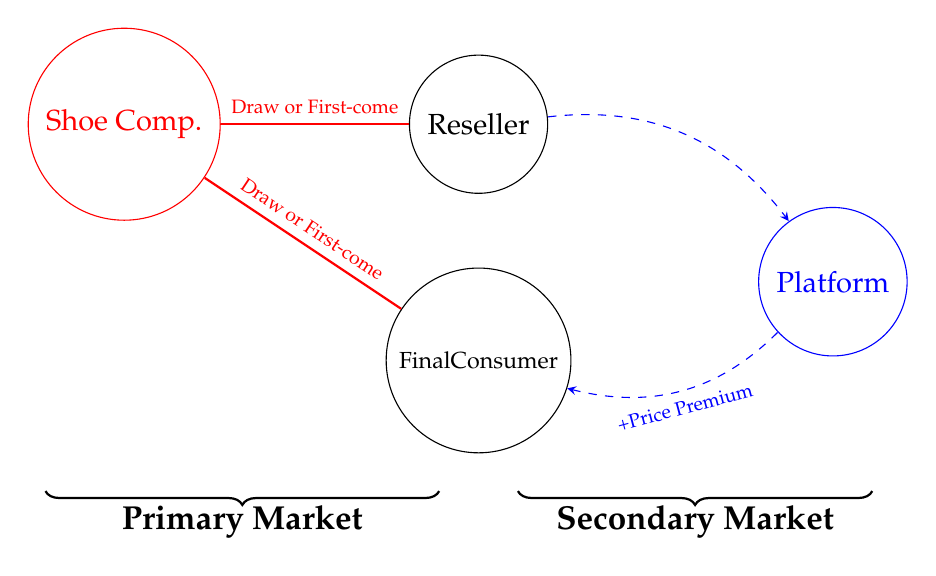
\begin{tikzpicture}[scale=.5,font=\scriptsize, sloped] %\tzhelplines(10,10)
		\tznode*[circle, scale=1.5, red](-1,0)(A){Shoe Comp.}
		\tznode*[circle, scale=1.5](8,0)(B){Reseller}
		\tznode*[circle, scale=1.2](8,-6)(C){FinalConsumer}
		\tznode*[circle, blue, scale=1.5](17,-4)(D){Platform}
		\tzline[thick, red](A){Draw or First-come}(B)
		\tzline[thick, red](A){Draw or First-come}(C)
		\tzto[->, bend  left, dashed, blue](B)(D)
		\tzto[->, bend  left, dashed, blue](D){+Price Premium}[below](C)
		\draw [thick, decorate,decoration={brace,amplitude=5pt,mirror,raise=4ex}]
		(-3,-8) -- (7,-8) node[midway,yshift=-3em]{\textbf{\large Primary Market}};
		\draw [thick, decorate,decoration={brace,amplitude=5pt,mirror,raise=4ex}]
		(9,-8) -- (18,-8) node[midway,yshift=-3em]{\textbf{\large Secondary Market}};
	\end{tikzpicture}
	\label{fig1:Figure1}
\end{figure}

In the secondary market, the transactions are usually completed at platforms such as `StockX'\footnote{(URL: \url{https://stockx.com})} and `GOAT'\footnote{(URL: \url{https://www.goat.com})} in the United States. The process of the secondary market is following:

\begin{itemize}
	\item A buyer in the secondary market has three choices
	\begin{enumerate}
		\item Bidding the price - wait until a seller chooses the bidding price
		\item Purchasing at the price of Ask - the purchase is completed in that moment
		\item Not purchase
	\end{enumerate}
	\item A seller in the secondary market has three choices
	\begin{enumerate}
		\item Asking the price - wait until a buyer chooses the asking price
		\item Selling at the price of Bid - the purchase is completed in that moment
		\item Not sell
	\end{enumerate}
\end{itemize}

Two players choice exercise the powers that draw prices down for buyers and up for sellers. Interestingly, both players have no information about the total quantity and the possibility of re-release from shoe companies. However, they can obtain the infromation: the list of current asking prices and bidding prices. Due to the option that the buyer and the seller just are able to click the purchase or sell button if they like the price, they are not fully informed; but, they can still have an access to previous short term price history. Briefly, both players can read trends and predict but not completely. This relationship between two players, I assume, is not hindered from shoe companies.

\subsection{Research Question}

In the literature of sequential auctions, researchers can find the price trends (\textcite{ashenfelter1992testing}, \textcite{ginsburgh1998absentee}, \textcite{deltas1999auction}, and \textcite{deltas2004catalogue}) and try to figure out the important factors which make the price trends. These results can also be shown in the data set I will use. From the basical data description, it is apparant that there is a decline pattern in price. Throughout the anlaysis of data sets and estimations, I want to asnwer the question that whether the price declining trend does exist and whether it has statistical significance in the sneaker market. Then, it is necessary to figure out the key-role factors to make the price patter either a decline or an increase.  \\

Therefore, the priority should be taken by the examination of a price pattern. I need to check it with the whole data and several subset of the data. The second question is whether the total number of transaction - large size market - has any impacts on the price convergence. This question is raisen by \textcite{deltas1999auction} to examine whether the price movement in large size auction markets seems competitive market's prices. 

However, the most important starting point is how to identify each auction. I consider each trasaction of a pair of sneaker as one auction sequentially takes place. The underlying assumption is each individual has their own foot size so that two sizes of sneakers cannot be interchangable even though they are the same sneaker. The colors are in the same assumption, which seems too strict. After the examination, this two assumptions can be relaxed, and I can check the inter-color and -size substitutability.

\section{Data}


Sellers can easily put their clohting stuffs such as shoe, sneakers, apparel, eletronics, etc. on the lists with asking prices, while buyers can list their bidding prices. By approaching StockX API, I can request very detail transaction data by products, size, time, and buyer's region. However, I faced authentication issue, having another way to get some data from `Kaggle'\footnote{URL: \url{www.kaggle.com}}. In this section, I will show details of data I could get from the `StockX data contest' in Kaggle.

\begin{table}[H]
	\centering
	\caption{Data Summary}
	\begin{tabular}{c|ccc}
		\hline\hline
		& $ N $ & min & max \\\hline
		Sneaker & 50  & 1  & 50   \\
		Saleprice & 99,956 & \$180 & \$4050 \\
		Retailprice & 220 & 130 & 250 \\
		Shoesize & 26 & 3.5 & 17  \\
		Order & 99,956 &  1 & 11,423 \\
		Month & 18 & 9/2017 & 2/2019 \\
		Region & 51 & & \\
		\hline\hline
	\end{tabular}
	\label{tab;table1}
\end{table}



Table \ref{tab2;table2} shows the detail summary statistics of retail and sale price variable. While the retail price has nigligible variation since the brands in the data set is limited, the sale price has a noticeable variation overtime. The most important measurement is time dimentional variable. I measured it as the order of transaction. This is because even though the data is recorded daily, some pairs traded more than one time per a day. 

\begin{table}[h]
	\centering
	\caption{Data Summary2}
	\begin{tabular}{c|ccccccc}
		\hline\hline
		& mean & sd & p10 & p25 & p50 & p75 & p90 \\\hline
		Retailprice & 208.6136  & 25.2000  & 160 & 220 & 220 & 220 & 220 \\
		Saleprice & 446.6347  & 255.983  & 250 & 275 & 370 & 540 & 750   \\
		\hline\hline
	\end{tabular}
	\label{tab;table2}
\end{table}

Table \ref{tab3;table3} shows the detail summary statistics for `order'. For the maximum value of `order' means the highest density sneaker has been traded 11,423 times.  In Figure \ref{fig2:fig2}, left figure stands for the distribution of `order', while the right figure explains the distribution of each pair in terms of `order'. Most of them have been traded less than 4000 times.

\begin{table}[H]
	\centering
	\caption{Data Summary3}
	\begin{tabular}{c|cccccccc}
		\hline\hline
		& mean & sd & p10 & p25 & p50 & p75 & p90 & Max \\\hline
		order & 3243.2 & 2960.0  & 217 & 656 & 2356 & 5148 & 8066 & 11423   \\
		\hline\hline
	\end{tabular}
	\label{tab3;table3}
\end{table}

\begin{figure}[h]
	\begin{subfigure}{0.5\textwidth}
		\centering
		\caption{Distribution of `order'}
		\includegraphics[width=0.9\linewidth]{Rplot.png}
	\end{subfigure}%
	\begin{subfigure}{0.5\textwidth}
		\centering
		\caption{Individual Sneakers Distribution of `order'}
		\includegraphics[width=0.9\linewidth]{order.png}
	\end{subfigure}
	\caption{Distribution of `order'}
	\label{fig2:fig2}
\end{figure}


\vspace{1cm}

\section{My Contribution}

First of all, my data set is unique to examine sequential auctions market. Taking advantage of E-commerce, I can see almost continuum transactions which are not regular. This characteristic is resulted from the low barrier to join this market. Second, in the conventional auction market, it is hard to find the identical goods with numerous numbers. However, in this market, the maximum number of transactions of identical item is almost 1,261 within 2 years\footnote{This number is calculated from the order of transaction with size consideration. See Table \ref{tab2;table2}}. Moreover, after this project, I would like to generate more variable and obtain more data, which leads me to be able to have more precise and interesting analysis. \\
The results from this project are consistent with the literature of sequential auction. Therefore, as some studies show the increasing pattern, I can also find the increasing pattern among the transactions. The another future steps should be the separate examination of increasing and decreasing patterns of prices.


\section{Models and Variables}

In this section, I introduce estimation models and variables.  

\subsection{Econometric Model}

To capture the price pattern, $ t $ is from now on regarded as the order of transaction. To distinguish the order from the order counted differently as size, I denote $ t $ and $ t_{s} $ respectively. 

\subsubsection{Using Size9.5-10 Data}

Given the size 9.5 and 10 are the most popular size for people, I, firstly, run a regression by using only 9.5-10 size shoes together. The interchangability of two similar sizes is underlying consideration. Also, since the data includes eighteen month length of time variation, month fixed effets are assigned. The regression equation is following:

\begin{equation}
	y_{it} = \beta_{1}t_{i} + \gamma_{m} + \delta_{i}
\end{equation}

\begin{align*}
	& y_{it} = \text{The ratio of Saleprice and Retailprice}\footnotemark  (\%) \\
	& t_{t} = \text{The order of transaction of sneaker $ i $} \\
	& \gamma_{m} = \text{Month fixed effects} \\
	& \delta_{i} = \text{Sneakers fixed effects}
\end{align*}

Due to the seasonality, I put $ \gamma_{m} $ as month fixed effects. For equation (1), I run a fixed effect regression.

\subsubsection{Using Whole Data}

In this section, to utilize the rich data set, I set up three equations.

\begin{equation}
	y_{it} = \beta_{1}t_{i} + \beta_{2}X_{1,it} + \beta_{3}X^{2}_{1,it} + \delta_{i} + \gamma_{m} + \varepsilon_{it}
\end{equation}

\begin{equation}
	y_{it} = \beta_{1}t_{i} + \beta_{2}X_{1,it} + \beta_{3}X^{2}_{1,it} + \delta_{i}+\gamma_{m} + R_{i} + \varepsilon_{it}
\end{equation}

\begin{equation}
	y_{it_{s}} = \beta_{1}t_{s,i} + \beta_{2}X_{1,it_{s}} + \beta_{3}X^{2}_{1,it_{s}} + \delta_{i}+\gamma_{m}  + \varepsilon_{it_{s}}
\end{equation}


\begin{align*}
	& y_{it} = \text{The ratio of Saleprice and Retailprice}\footnotemark  (\%) \\
	& t_{i} = \text{The order of transaction of sneaker $ i $} \\
	& t_{s,i} = \text{The order of transaction of sneaker $ i $ size $ s $} \\
	& \gamma_{m} = \text{Month fixed effects} \\
	& \delta_{i} = \text{Sneakers fixed effects} \\
	& R = \text{Regional dummies} \\
\end{align*}

\addtocounter{footnote}{-1}
\footnotetext{A Saleprice means the price of a secondary market, and a Retailprice means the price of a primary market which is fixed. }

\addtocounter{footnote}{1}
\footnotetext{I show the validity of the square term of shoe size in Appendix A}



\subsection{Variable Description}

\subsubsection{Transaction Variable}

Every variable, sub-indexed by $ t $, contains the information what order the transaction has made. This is because several sneakers were traded within a day, and there is no specific `time' information to capture the detail order. Almost a half of total transactions are in that case. This would be another potential factors because if it is seen for buyers, it could be the pressure to lose the chance to buy it. Within this paper, I just assume that the transactions were recorded as time order so the order I assign is reliable. I have two ways to make this variable; first, just by sneakers with coloer, second, by sneakers with color and sizes.

\begin{table}[H]
	\centering
	\caption{Data Summary}
	\begin{tabular}{c|ccc}
		\hline\hline
		& $ N $ & min & max \\\hline
		$ t $ & 99,956  & 1  & 11,423   \\
		$ t_{s} $ & 99,956 & 1 & 1,261 \\
		\hline\hline
	\end{tabular}
	\label{tab4;table4}
\end{table}

\subsubsection{The Ratio of Saleprice and Retailprice}

In the data, eleven types of sneakers without consideration of color variation have their own retailprices. None of them has winning bid at the lower prices than the retailprices. Thus, I calculate the ratio with percentage so that I can see the price pattern as the percentage of price premium.

\begin{table}[H]
	\centering
	\caption{Data Summary}
	\begin{tabular}{c|ccc}
		\hline\hline
		& $ N $ & min & max \\\hline
		Ratio(\%) & 99,956  & 84.54  & 2131.57   \\
		\hline\hline
	\end{tabular}
	\label{tab5;table5}
\end{table}


%\subsubsection{The Number of Transactions}

%This variable is generated in order to examine the importance of size of markets. As I do in transaction variable, I have two ways to count the number of transactions whether I consider the size variation.
\section{Results}

\subsection{Fixed Effects Estimation}

\begin{table}[H]
	\centering
	\caption{Estimation Result}
	\begin{tabular}{p{0.13\textwidth}p{0.17\textwidth}p{0.17\textwidth}p{0.17\textwidth}p{0.15\textwidth}}
		\hline \hline
		& (1) & (2) & (3) & (4)  \\
		& Price ratio\% & Price ratio\% & Price ratio\% & Price ratio\%  \\ \hline
		Order        &      -0.008***&      -0.006*** & -0.006*** & \\
		&     (0.000)   &     (0.000) & (0.000)  &    \\
		Order$_{s}$ & & & &  -0.010*** \\
		&&&& (0.000) \\[0.2cm]
		shoesize            &       &       1.389***  & 1.475***  &  2.679***\\
		&        &     (0.002) & (0.001) & (0.000)  \\
		shoesize$^{2}$         &      Fix Size9.5-10 &      -0.054* & -0.0553** & -0.111*** \\
		&        &     (0.026) & (0.024) & (0.000)   \\
		&&&&\\
		Region FE & & Not Significant & & \\
		\hline
		Sneakers FE      & \checkmark & \checkmark & \checkmark & \checkmark \\
		Month FE & \checkmark & \checkmark & \checkmark & \checkmark \\
		Observations        &      19,778  &      99,956  & 99,956 & 99,956 \\
		Adjusted $ R^{2} $  &       0.966   &   0.959 & 0.964 & 0.963  \\
		\hline\hline
	\end{tabular}
	\label{tab6:table6}
\end{table}

Table \ref{tab6:table6} shows the estimation result of equation (1) to (4). All of the interesting coefficient (Order) shows consistently negative sign. Also they are statistically significant and have high explanatory power. The first research question can be answered: there is a decreasing price trend. This implies consumers in this market shows risk aversion. As the social medias are expanding and getting popular for young generations who are the main consumers in this market, consumers do not want to miss those popular sneakers. The following result convinces this statement more robust.

\begin{table}[H]
	\centering
	\caption{Magnitude of Declining}
	\begin{tabular}{c|cccccc}
		\hline\hline
		& 1-10th & 10th-20th & 20-30th & 40th-50th & $ \cdots$ & 90-110th \\\hline
		order & -12.02  & -3.89  & -2.54 & -1.57 & $ \cdots$& -0.14   \\
		\hline\hline
	\end{tabular}
	\label{tab7;table7}
\end{table}

According to Table \ref{tab7;table7}, it is precise that the magnititude of declining cools down. When I talked with an undergraduate student, the student commented `hyped-down' trend in this market. If one is not able to buy the popular sneakers quickly, the value of sneakers would not remain longer. Therefore, consumers would like to buy it at the beginning of the market. \\
For column (1) - (3), they are alike. In column (2), the buyer's regional fixed effect does not significant so I drop it for the other estimations. The interesting thing is column(4). If I disginguished size from size, it can be seen that the negative effect is twice larger in absolute value. It may be interpreted that certain shoe size such as 9.5-10 have more strong price pattern. 

\vspace{1cm}


\section{Discussion and Concluding Remarks}


From Table \ref{tab6:table6} , we can find the statistically significant coefficient of daily variable. This implies that the sequence of each auction shows decreasing price trend. Even though there is a data limiatation, 99,956 number of data is rich enough to look at this market's tendency. For the future work, I can gather the number of bidders and askers to examine how the power of each player plays a role in this market and what the number of bidders and askers does mean.

\newpage

\printbibliography

\newpage
\begin{appendices}
	\section*{Appendix A}
	
	
	\subsection*{Simple Regression}
	
	I do regression `saleprice' on `shoe size' as following
	\begin{equation}
		y_{it} = \beta_{1}x_{it} - \beta_{2}x_{it}^{2} + \gamma_{i} + \varepsilon_{i}
	\end{equation}
	According to the StockX data graphs and summary statistics, it is rational to run a regression with square term with sneakers specific fixed effect.
	
	\begin{table}[H]
		\centering
		\caption{Simple Regression Result}
		\begin{tabular}{p{0.2\textwidth}p{0.1\textwidth}}
			\hline \hline
			Dependent Var & saleprice \\ \hline
			shoesize            &      27.081***\\
			&     (0.890)   \\
			shoesize2           &      -1.357***\\
			&     (0.050)   \\
			Observations        &      99,956   \\
			\hline\hline
		\end{tabular}
	\end{table}
\end{appendices}










	
\end{large}
\end{document}